\documentclass[12pt, french]{article}

\usepackage{fancyhdr, fancybox, lastpage,mhchem, mathrsfs, tikz}
\usepackage[most]{tcolorbox}
\usepackage[a4paper, margin={0.3in, .75in}]{geometry}
\usepackage{wrapfig}
\pagestyle{fancy}
\renewcommand\headrulewidth{1pt}
\renewcommand\footrulewidth{1pt}
\fancyhf{}
\rhead{ \em{Zakaria Haouzan}}
\lhead[C]{\em{2ème année baccalauréat Sciences Physiques}}
\chead[C]{}
\rfoot[C]{}
\lfoot[R]{}
\cfoot[]{\em{Page \thepage / \pageref{LastPage}}}


\newtcolorbox{Box2}[2][
enhanced, 
    breakable,
]{
                lower separated=false,
                colback=white,
colframe=white!20!black,fonttitle=\bfseries,
colbacktitle=white!30!gray,
coltitle=black,
enhanced,
attach boxed title to top left={yshift=-0.1in,xshift=0.15in},
title=#2,#1}


\begin{document}
\begin{center}
   \shadowbox {\bf{Chute verticale}
 }

\end{center}

\vspace{-0.2cm}
%%_________________________Exercice ! :"_________________________Exercice
   \begin{Box2}{Exercice 1 : Mouvement d’un solide dans le champ de pesanteur }


	   \begin{wrapfigure}[12]{r}{0.3\textwidth}   
  \begin{center}
	  \vspace{-0.6cm}
	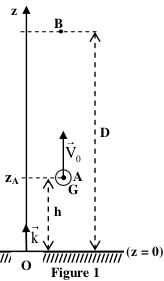
\includegraphics[width=0.2\textwidth]{./ex_00_0.png}
	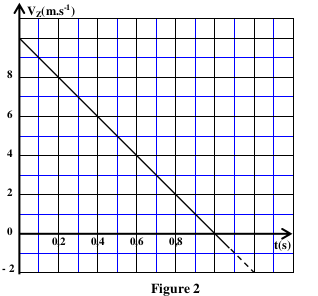
\includegraphics[width=0.355\textwidth]{./ex_00_1.png}
  \end{center}
\end{wrapfigure}

	   \textbf{\underline{Partie 1 : }}
	   \emph{L’étude des mouvements des solides dans le champ de pesanteur uniforme permet de déterminer les
grandeurs caractéristiques de ces mouvements.
L’objectif de cette partie de l’exercice est d’étudier le mouvement d’une balle dans le champ de
pesanteur uniforme.}

On lance verticalement vers le haut avec une vitesse initiale $\vec{V_0}$ , à un 
 instant choisi comme origine des dates $(t=0)$ , une balle de masse m d’un
point A situé à une hauteur $h = 1,2 m$ du sol.
On étudie le mouvement du centre d’inertie G de la balle dans un
référentiel terrestre considéré galiléen. On repère la position de G,
à un instant t, dans le repère $(O , \vec{k})$ par la cote z ( Figure 1).

On considère que les forces de frottement et la poussée d’Archimède sont
négligeables.

\begin{enumerate}
	\item Définir la chute libre.
	\item En appliquant la deuxième loi de Newton, établir l’équation
\\différentielle vérifiée par la vitesse Vz du centre d’inertie G.
\item Monter que l’équation horaire du mouvement de G s’écrit :\\$z = -\frac{1}{2}g.t^2 +V_0.t + h $
\item La courbe de la figure 2 représente les variations de
la vitesse \\$V_z$ en fonction du temps.
En exploitant le graphe de la figure 2, \\écrire
l’expression numérique de la vitesse $V_z = f(t)$.
\item Le centre d’inertie G passe, au cours de la montée,
	par le point B situé à une \\hauteur D du sol, avec une vitesse $V_B = 3m.s^{-1}$ (figure1). Montrer que   $D =5,75m$ .
\item  On lance de nouveau, à un instant choisi comme
nouvelle origine des dates (t=0) , verticalement vers le
haut, la balle du même point A avec une vitesse
initiale $V' =8m.s^{-1}$ . Le centre d’inertie G de la balle
atteint-il le point B? Justifier votre réponse.

\end{enumerate}

\textbf{\underline{Partie 2 : Etude de la chute avec frottements  }}
Pour ne pas se détériorer lors du choc avec le sol, un paquet d’aliments a été attachée
à un parachute lui permettant une descente lente. L’hélicoptère reste immobile à une
altitude H au-dessus du point O. Le paquet et son parachute tombent verticalement
sans vitesse initiale à l’instant $t_0 = 0$.
L’air exerce des forces de frottements modélisées par la relation : $\vec{f}$=$-100.\vec{v}$ , où $\vec{v}$
représente le vecteur vitesse du paquet à l’instant t.
On néglige la poussée d’Archimède pendant la chute.

\textbf{On donne : } La masse du système {caisse + parachute} : $m = 150 kg$.
  
\begin{center}
	  \vspace{-0.2cm}
	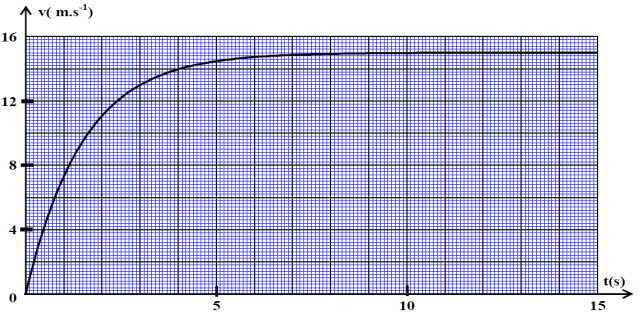
\includegraphics[width=0.61\textwidth]{./ex_00_2.png}
  \end{center}
\begin{enumerate}

	\item[7.] Etablir l’équation différentielle vérifiée par la vitesse du centre d’inertie $G_1$ du
		système dans le repère $(R,O,\vec{i}, \vec{j})$ .

	\item[8.] La courbe de la figure 2, représente les variations de la vitesse du centre
d’inertie $G_1$ du système en fonction du temps. Déterminer la valeur de la vitesse
limite $V_{lim}$ et celle du temps caractéristique $\tau$ de chute.
\item[9.] Estimer la durée du régime initial.
\item[10.]  Par utilisation de la méthode d’Euler et le tableau suivant, déterminer les valeurs
de la vitesse $v_4$ et de l’accélération $a_4$.


\end{enumerate}

\begin{center}
\begin{tabular}{ |c|c|c|c|c|c|c|c| } 
 \hline
 $t_i(s)$		 & 0&0,1 &0,2& 0,3& 0,4& 0,5& 0,6\\\hline
 $V_i(m/s)$      &0 & 1,0 & 1,93 & 2,80 &$v_4$&4,37&5,08\\\hline 
 $a_i(m.s^{-2})$ & 10,0& 9,33 & 8,71 &8,12&$a_4$&7,07& 6,60\\\hline  
 \hline
\end{tabular}
\end{center}
% Required package
 
 
 
   \end{Box2}


%%_________________________Exercice !2 :"_________________________Exercice
\begin{Box2}{Exercice 2 :Les toboggans }
	\begin{wrapfigure}[6]{r}{0.5\textwidth}
  \begin{center}
	  \vspace{-0.6cm}
	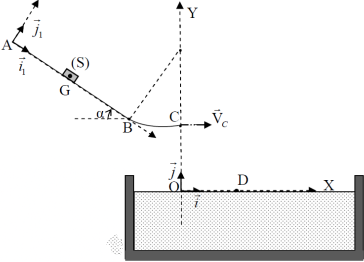
\includegraphics[width=0.52\textwidth]{./ex_01_0.png}
  \end{center}
\end{wrapfigure}

	\emph{Les toboggans dans les piscines permettent aux nageurs de glisser et de plonger
dans l’eau.
On modélise un toboggan par une piste ABC constituée d’une partie AB inclinée
d’un angle $\alpha$ par rapport au plan horizontal et d’une partie circulaire BC, et on
modélise le nageur par un solide (S) de centre d’inertie G et de masse m (Figure1).}

\textbf{Données :} AB = 2,4m ; $\alpha = 20^{\circ}$ ; $ g= 9,8m.s^{-2}$ ; m = 70Kg.

\textbf{Etude du mouvement vertical de G dans l’eau :}
Le solide \\(S) poursuit son mouvement dans
l’eau, avec une vitesse verticale V.\\ Il subit
en plus de son poids à :

\begin{itemize}
	\item Une force de frottement fluide
modélisée dans le système
\\international d’unité par : $\vec{f} =140.V^2.\vec{j^2}$

\item La poussée d’Archimède FA d’intensité $F_A = 637 N$.

\end{itemize}
On considère l’instant d’entrée de (S) dans l’eau comme nouvelle origine des temps.

\begin{enumerate}
	\item Montrer que la vitesse V(t) de G vérifie l’équation différentielle suivante : $$\frac{dV(t)}{dt}-2.V^2 + 0,7 = 0$$

	\item Trouver la valeur de la vitesse limite $V_l$.
	\item Déterminer à l’aide du tableau suivant, et par utilisation de la méthode
		d’Euler, les valeurs : $a_{i+1}$ et $V_{i+2}$.
\end{enumerate}

\begin{center}
\begin{tabular}{ |c|c|c| } 
 \hline
 $t(s)$		& $V(m.s^{-1})$	 & $a(m.s^{-2})$ \\\hline
 $t_i = 1,8.10^{-1}$		& $-1,90$		& 6,52 \\\hline 
 $t_{i+1}= 1,95.10^{-1}$	& -1,80	& $a_{i+1}$ \\\hline  
 $t_{i+2}= 2,1.10^{-1}$	& $V_{i+2}$	& 5,15 \\\hline  
 \hline
\end{tabular}
\end{center}
\end{Box2}

\begin{center}
   \Large{ \em{Exercices Supplémentaires}}
\end{center}


\begin{Box2}{Exercice 3 :liquide visqueux  }
	
	\begin{wrapfigure}[2]{r}{0.52\textwidth}
  \begin{center}
	  \vspace{-0.6cm}
	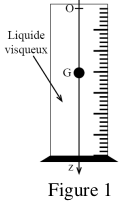
\includegraphics[width=0.17\textwidth]{./ex_02_1.png}
	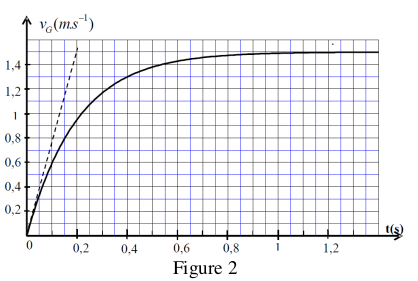
\includegraphics[width=0.52\textwidth]{./ex_02_02.png}
  \end{center}
\end{wrapfigure}


	\emph{L’étude de la chute d’un solide homogène dans un liquide visqueux permet de
déterminer quelques caractéristiques cinétiques et la viscosité du liquide utilisé.}

On remplit un tube gradué par un liquide visqueux, transparent et
de \\masse volumique $\rho$, puis on y laisse tomber, sans vitesse
initiale, à \\l’instant $t = 0$, une bille homogène de masse m, et de
centre d’inertie G.

On étudie le mouvement de G par rapport à un repère terrestre
supposé \\galiléen.
La position de G est repérée à un instant t, par l’ordonnée z, \\sur
l’axe $(\vec{Oz})$ vertical descendant (Figure 1).

On considère que la position de G est confondue avec l’origine de l’axe (Oz) à
l’instant $t = 0$, et que la poussée d’Archimède $\vec{F}$ n’est pas \\négligeable par rapport aux
autres forces \\appliquées sur la bille.
On modélise l’action du \\liquide sur la bille au cours du mouvement par \\une force de
frottement : $\vec{f} = - k.\vec{v_G}$ .

$v_G$ est la vitesse de G à un instant t, et k un \\facteur constant et positif.

\textbf{Données : }  Rayon de la bille : $r = 6,00.10^{-3} m$
 \\Masse de la bille : $m = 4,10.10^{-3}kg$

On rappelle que l’intensité de la poussée \\d’Archimède est égale au poids du liquide
déplacé.

\begin{enumerate}
	\item Par application de la deuxième loi de Newton, montrer que l’équation
		différentielle du mouvement de G s’écrit sous la forme : $\frac{dv_G}{dt} + A.v_G = B$ , en exprimant A en fonction de k et m, et
pesanteur), m, $\rho$ et V (volume de la bille).

\item Vérifier que l’expression : $v_G = \frac{B}{A}\big{(}1-e^{\frac{-t}{\tau}} \big{)}$ est solution de l’équation différentielle, où $\tau = \frac{1}{A}$ est le temps caractéristique du mouvement.

\item Ecrire l’expression de la vitesse limite $V_{lim}$ du centre d’inertie de la bille en
fonction de A et B.

\item On obtient, à l’aide d’un
matériel informatique
convenable, la courbe de
la figure 2, représentant
les variations de la vitesse
$v_G$ en fonction du temps.
Déterminer graphiquement
les valeurs de $V_{lim}$ et $\tau$.

\item Déterminer la valeur du coefficient k. 
\item Le coefficient k varie avec le rayon de la bille et la viscosité $\eta$ du liquide selon
la relation suivante : $k = 6\pi.\eta.r$.
Déterminer la valeur de $\eta$ du liquide utilisé dans cette expérience.

\item L’équation différentielle du mouvement de G s’écrit sous la forme :
$\frac{dv_G}{dt} = 7,57 - 5.v_G$ . Par application de la méthode d’Euler, et les données du

tableau, déterminer les valeurs de $a_1$ et $v_2$.
\end{enumerate}

\begin{center}
\begin{tabular}{ |c|c|c| } 
 \hline
 $t(s)$		& $V(m.s^{-1})$	 & $a(m.s^{-2})$ \\\hline
 $0$		& $0$		& 7,57 \\\hline 
 $0,033$	& 0,25	& $a_1$ \\\hline  
 $0,066$	& $V_{2}$	& 5,27 \\\hline  
 \hline
\end{tabular}
\end{center}


\end{Box2}
	%\vspace{-0.8cm}


\begin{Box2}{Exercice 4 :Etude du mouvement d’une charge }
	\begin{wrapfigure}[13]{r}{0.32\textwidth}
  \begin{center}
	  \vspace{-0.6cm}
	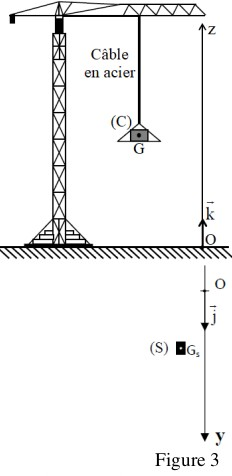
\includegraphics[width=0.32\textwidth]{./ex_03_00.jpg}
  \end{center}
\end{wrapfigure}


	\textbf{Première partie : Etude du mouvement d’une charge }
Les grues sont utilisées dans les chantiers de construction, pour lever les charges
lourdes, à l’aide des câbles en acier liés à des dispositifs spéciaux.
Le but de cet exercice est l’étude du mouvement
vertical d’une charge, puis l’étude de la chute
verticale d’une partie de cette charge dans l’air.
On prendra g = 9,8 m.s-2.

\textbf{Partie 2 : Chute verticale dans l’air d’une partie de
la charge :}

La charge s’arrête à une altitude donnée. A un
instant $t = 0$, une partie (S) de cette charge, de
masse $m_S = 30 kg$, tombe sans vitesse initiale.
On étudie le mouvement du centre d’inertie $G_S$
de la partie (S) dans
le repère (O, j) où l’axe (Oy) est vertical
descendant (Figure 3).
La position de $G_S$ Coïncide avec l’origine du repère (Oy) à l’origine
des temps.
On modélise l’action de l’air sur la partie (S) au cours de son
mouvement \\par la force :
un instant t et $k = 2,7 (SI)$. $\vec{f} = -k.v^2 .\vec{j}$ , où $\vec{v}$ le vecteur vitesse de $G_S$ à
On \\néglige l’action de la poussée d’Archimède devant les autres
forces appliquées à (S).

\begin{enumerate}

	\item Déterminer, par analyse dimentionnelle, l’unité de la
constante k dans le système \\international.

\item Montrer que l’équation différentielle verifiée par la vitesse v s’écrit comme suit : $$\frac{dv}{dt}+9.10^{-2}.v^2 = 9,8$$

\item Déterminer la vitesse limite $V_{lim}$ du mouvement.
\item Sachant que la vitesse du centre d’inertie $G_S$ à un instant $t_1$ est $v_1$ =$2,75 m.s^{-1}$,
trouver, par application de la méthode d’Euler, la vitesse $v_2$ à l’instant
$t_2 = t_1 + \Delta{t}$, sachant que la pas du calcul est $\Delta{t} = 2,4.10^{-2}s$.

\end{enumerate}
\end{Box2}




%\begin{Box2}{Exercice 5 : Cas d'un mouvement curviligne (utilisation du repère de Frenet) : }

%%\begin{wrapfigure}[3]{r}{0.33\textwidth}
	%%\vspace{-0.8cm}

%\end{Box2}

%\vspace{-0.8cm}

%%%_________________________Exercice ! 3:"_________________________Exercice
%\begin{Box2}{Exercice 6: La synthèse }
%%\begin{wrapfigure}{r}{0.4\textwidth}
  %%\begin{center}
	%%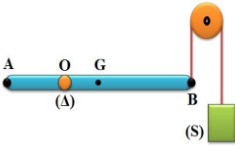
\includegraphics[width=0.4\textwidth]{./ex02.png}
  %%\end{center}
%%\end{wrapfigure}

%\end{Box2}

%%%_________________________Exercice 4 : _________________________Exercice
%\begin{Box2}{Exercice 7 :Le ski }
   %% \begin{wrapfigure}[12]{r}{0.5\textwidth}

%%\end{wrapfigure}

%\end{Box2}

\begin{center} 
	\emph{\textbf{” If you cannot do great things, do small things in a great way.” ~ Napoleon Hill.}}
\end{center}

%\vspace{-0.6cm}
%%%_________________________Exercice 5 : _________________________Exercice
%\begin{Box2}{Exercice 4 : }
   %% \begin{wrapfigure}[14]{r}{0.5\textwidth}
  %%\begin{center}
	  %%\vspace{-0.6cm}
	%%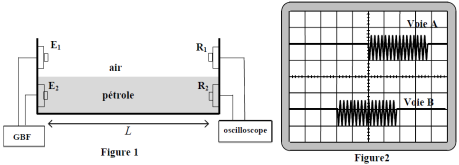
\includegraphics[width=0.5\textwidth]{./img/ex5.png}
  %%\end{center}
%%\end{wrapfigure}

%4

%\end{Box2}

%\begin{Box2}{Exercice 5 : }

%44
%\end{Box2}


%\begin{Box2}{Exercice 6 : }


	%\end{Box2}


%\begin{Box2}{Exercice 7 : }
%\end{Box2}
\end{document}
